\documentclass[11pt,a4paper]{article}
\usepackage{fontspec}
\setmainfont{DejaVu Serif}[Scale=0.92]
\setsansfont{DejaVu Sans}[Scale=0.92]
\newfontfamily\cjk{Noto Serif CJK TC}
\usepackage{graphicx}
\usepackage{xcolor}
\usepackage{geometry}
\usepackage{amsmath}
\usepackage{booktabs}
\usepackage{tabularx}
\usepackage{colortbl}
\usepackage{enumitem}
\usepackage{titlesec}
\usepackage{fancyhdr}
\usepackage{caption}
\usepackage{ragged2e}
\usepackage[most]{tcolorbox}
\usepackage[numbers,super,sort&compress]{natbib}
\geometry{a4paper, top=2.4cm, bottom=2.6cm, left=2.4cm, right=2.4cm}
\definecolor{ink}{HTML}{1A3A4A}
\definecolor{accent}{HTML}{B8433A}
\definecolor{steel}{HTML}{1A6B8A}
\definecolor{mist}{HTML}{9DB4C0}
\definecolor{gold}{HTML}{8A6D1A}
\definecolor{rowgray}{HTML}{F5F6F7}
\definecolor{fieldgray}{HTML}{6B7B85}
\titleformat{\section}{\Large\bfseries\color{ink}}{\thesection}{0.7em}{}[\vspace{1pt}{\color{ink}\titlerule[1.1pt]}]
\titleformat{\subsection}{\large\bfseries\color{ink}}{\thesubsection}{0.6em}{}
\titlespacing{\section}{0pt}{15pt}{7pt}
\titlespacing{\subsection}{0pt}{11pt}{4pt}
\pagestyle{fancy}\fancyhf{}
\fancyhead[C]{\footnotesize\color{gray}CarbonPass --- Project Proposal, 2026 Presidential Hackathon International Track}
\fancyfoot[C]{\footnotesize\thepage}
\renewcommand{\headrulewidth}{0.3pt}
\captionsetup{font=small,labelfont=bf,justification=raggedright,singlelinecheck=false}
\renewcommand{\arraystretch}{1.25}
\setlength{\parskip}{4.2pt}\setlength{\parindent}{0pt}
\newtcolorbox{formfield}[1]{enhanced,breakable,colback=rowgray,colframe=rowgray,
  left=9pt,right=8pt,top=6pt,bottom=6pt,arc=1.5pt,boxrule=0pt,
  borderline west={2.6pt}{0pt}{steel},
  before upper={\textbf{\textcolor{fieldgray}{\footnotesize\MakeUppercase{#1}}}\par\vspace{2pt}},
  before skip=8pt,after skip=8pt}
\newtcolorbox{spotlight}[1]{enhanced,breakable,colback=white,colframe=white,
  borderline west={2.6pt}{0pt}{accent},left=8pt,right=4pt,top=3pt,bottom=3pt,
  before upper={\textbf{\textcolor{accent}{#1}}\quad},arc=0pt,boxrule=0pt,
  frame hidden,before skip=7pt,after skip=7pt}
\newcommand{\NT}{NT\$}
\usepackage[colorlinks=true,linkcolor=steel,citecolor=ink,urlcolor=steel,
  bookmarks=true,bookmarksnumbered=true,unicode=true]{hyperref}

\begin{document}

% ===== COVER =====
\begin{titlepage}
\newgeometry{margin=0cm}
\noindent
\begin{minipage}{\textwidth}
{\color{ink}\rule{\textwidth}{14mm}}\\[-2.5pt]
{\color{accent}\rule{\textwidth}{2.6mm}}
\end{minipage}
\vspace{2.3cm}
\begin{minipage}{0.9\textwidth}
\hspace{1.8cm}\begin{minipage}{0.9\textwidth}
{\sffamily\footnotesize\bfseries\color{accent}\MakeUppercase{P r o j e c t\ \ P r o p o s a l\ \ ·\ \ I n t e r n a t i o n a l\ \ T r a c k}}\\[8mm]
{\fontsize{31}{35}\selectfont\bfseries\color{ink}CarbonPass}\\[4mm]
{\Large\color{ink!80}The waste nobody measures}\\[6mm]
{\normalsize\color{black!68}One photograph becomes a small factory's EU carbon report --- and the\\carbon-and-cash map of the steel it throws away. An AI that runs offline,\\on a laptop, on the excluded side of the wall.}\\[12mm]
{\color{ink}\rule{2.6pt}{3.1cm}}\hspace{4mm}%
\begin{minipage}[b]{0.82\textwidth}\small
2026 Presidential Hackathon --- International Track\\[1.5pt]
Theme: ``Digital Inclusion in the AI Era''\\[1.5pt]
Corresponding SDGs: 8 · 9 · 12 · 13\\[1.5pt]
Beachhead: fastener cluster (CN 7318), Gangshan--Luzhu, Kaohsiung\\[1.5pt]
Submission window: 22 May -- 31 July 2026
\end{minipage}
\end{minipage}
\end{minipage}
\vfill
\noindent
\begin{minipage}{\textwidth}
\hspace{1.8cm}\begin{minipage}{0.6\textwidth}
\footnotesize\color{black!55}
Every quantitative claim is either derived from the EU's own adopted
regulation or measured by our working engine and reproducible from the
repository. Estimates are labelled; synthetic magnitudes are flagged as
pending the pilot. All content is in English.
\end{minipage}
\hfill
\raisebox{-0.4cm}{{\color{mist}\rule{3cm}{3cm}}}\hspace{-3cm}\raisebox{-3.42cm}{{\color{ink}\rule{6.2cm}{3cm}}}
\end{minipage}
\restoregeometry
\end{titlepage}

\thispagestyle{plain}
{\hypersetup{linkcolor=ink}\tableofcontents}
\clearpage

% ===== EXECUTIVE SUMMARY =====
\section*{Executive Summary}
\addcontentsline{toc}{section}{Executive Summary}

Since 1 January 2026 an EU importer of steel fasteners must declare the carbon embedded in the goods --- and the regulation counts the mass of steel \emph{entering} the process, before any metal is cut away\cite{qa}. Every fastener factory in our study buys about \textbf{1.10 tonnes of steel for each tonne of product it ships}. The other \textbf{0.10 tonne is scrap} --- roughly a tenth of the steel, thrown in a skip --- and because CBAM counts the steel that goes in, that scrap is \emph{already inside the declared carbon number whether the owner looks at it or not}.

Nobody looks at it. Seeing it means reconciling a year of steel invoices against a production log, per product, per customs code --- an ERP-and-sustainability-team job that every large manufacturer already automates and that a thirty-person family factory has never once performed. That capability gap is the digital divide this project closes.

\textbf{CarbonPass turns one photograph into two things.} An owner photographs a Taipower electricity bill and steel e-invoices inside LINE; an AI that runs \emph{offline on a laptop} --- a four-billion-parameter model that read a Traditional-Chinese utility bill at 100\% field accuracy across six phone-photo degradations in our tests\cite{repo} --- returns (1) the verifier-ready EU CBAM data pack the buyer asks for, and (2) a \textbf{waste map}: the carbon and the cash sitting in the scrap bin, per product line, and what tightening the yield is worth. For our lead firm the engine measured \textbf{758 tCO$_2$e and \NT7.35\,million binned each year}; improving yield from 9.1\% to 5\% loss recovers \textbf{359 tCO$_2$e --- eighty times the carbon of the grid-scheduling module we also built}, and unlike scheduling it \emph{moves the CBAM number itself}\cite{repo}.

The pivot is deliberate and evidence-led. Our own engine, run against the EU's adopted default-value tables, killed the alarmist framing this project began with: Taiwan's carbon-steel default is \emph{mild} (\,$\approx$€224/t\,), far below China (\,$\approx$€528/t\,) or Indonesia (\,$\approx$€682/t\,)\cite{ir2621,repo}. Filing alone is worth only about €4/t to a Taiwanese carbon-steel maker\cite{repo}. So we stopped selling the filing. The compliance pack is the door the buyer opens; the waste it exposes is the value the owner keeps --- true and worth acting on \emph{whatever he files}. The same scan also surfaced a problem Taiwan cannot currently see: its stainless fasteners are among the most carbon-intensive on earth, yet the EU assigns them a carbon-steel default, so honest reporting would cost the buyer far more and nobody reports it (\S2.3). Taiwan is the proving ground for an instrument built to travel: the factories that need it most --- across ASEAN and South Asia --- are the ones with no cloud, no GPU, and no seat at the EU's accreditation table.

% ===== 1 TEAM =====
\section{Team Information}\label{sec:team}
\emph{Application form field 1. Member names, nationalities, contact emails, phone numbers, gender and current country of residence are entered in the online form; primary and secondary contacts listed first.}
\begin{formfield}{Composition and eligibility}
Three to ten members including at least one non-ROC national; two designated contacts; all materials in English\cite{handbook}. Competencies: machine-learning / document intelligence; energy-systems and optimisation; EU--Taiwan carbon-regulation analysis; fastener-industry domain knowledge. The entry is original work for this competition; the team commits to mentorship, implementation-result presentations and follow-up benefit tracking.
\end{formfield}

% ===== 2 PROJECT =====
\section{Project Information}\label{sec:project}

\subsection{Project name and introduction}
\textbf{Project name: CarbonPass --- a local-first AI that finds the carbon and cash a small factory throws away, using the same documents that file its EU carbon report.}

The user experience is one sentence: \emph{photograph your electricity bill and steel invoices in LINE, and receive both the CBAM data pack your European buyer needs and a map of the money and carbon in your scrap.} The compliance artifact opens the door; the waste map is the product.

\begin{formfield}{Detailed description of AI usage (application form field 2.2)}
CarbonPass is an AI system, not a form-filler. (1) \textbf{Document intelligence:} an open vision-language model (\texttt{qwen3-vl}, Apache-2.0) parses photographed, mixed-language, real-world documents --- Taipower bills, Ministry of Finance e-invoices (電子發票), production logs --- into structured activity data, resolving the ROC calendar ({\cjk 民國}) and Traditional-Chinese layouts. In our tests the \textbf{4-billion-parameter} tier reached \textbf{100\% field accuracy across six phone-photo degradations (tilt, blur, low light, JPEG, warp, combined) at 18--31 s/document, entirely offline on a laptop with no GPU}\cite{repo}. (2) \textbf{An allocation engine} (constrained optimisation with Monte-Carlo uncertainty) splits facility energy and steel across product lines and customs codes. (3) \textbf{A compliance rules engine} encodes the EU methodology\cite{ir2547} and default-value tables\cite{ir2621}, reproducing the Commission's own worked ``screws and nuts'' example to a relative error of $10^{-9}$\cite{repo}. (4) \textbf{A waste analyser} derives yield loss --- and the carbon and cash in it --- directly from the same activity data. The architecture is \textbf{local-first}: parsing and computation run on the factory's own device; only the outputs the owner chooses to send ever leave.
\end{formfield}

\subsection{Corresponding SDGs}
\textbf{SDG 12 (Responsible Production)} --- the core: measuring and cutting material waste, not merely accounting for it. \textbf{SDG 13 (Climate Action)} --- yield improvement removes real tonnes and lowers the declared product carbon. \textbf{SDG 9 (Industry \& Innovation)} --- giving traditional SMEs a capability corporations automated twenty years ago. \textbf{SDG 8 (Decent Work)} --- protecting a nameable export cluster's competitiveness.

\subsection{The problem to be resolved and its importance}\label{sec:problem}

\subsubsection*{The waste is already inside the number}
CBAM makes the fastener maker declare the carbon of the steel it \emph{buys}, and the methodology counts ``the mass of precursors as entering the production process (before cutting)''\cite{qa}. So the specific embedded emissions of a fastener decompose exactly:
\[
\mathrm{SEE_{direct}} \;=\; \frac{\text{own process emissions}}{\text{product tonnes}} \;+\; \underbrace{\frac{\text{steel in}}{\text{product out}}}_{\text{the ratio}}\times \mathrm{SEE_{steel}}
\qquad\Rightarrow\qquad
\Delta\mathrm{SEE} = \Delta(\text{ratio})\times \mathrm{SEE_{steel}}.
\]
No allocation model, no assumption: the yield ratio \emph{is} the dominant term. Measured by our engine from documents the pipeline already reads --- steel mass and unit price from the e-invoice XML, output tonnes from the production log --- three product lines across two firms bin the quantities in Table~\ref{tab:waste} and Figure~\ref{fig:waste}.

\begin{table}[htbp]
\caption{Yield loss measured from real document formats (synthetic corpus; mechanism exact, magnitude pending pilot)}
\label{tab:waste}
\small
\begin{tabularx}{\textwidth}{@{}lXrrrrr@{}}
\toprule
\textbf{Firm / line} & \textbf{Steel in} & \textbf{Out} & \textbf{Scrap} & \textbf{Loss} & \textbf{tCO$_2$e/yr} & \textbf{\NT/yr} \\
\midrule
Firm A --- carbon screws & 3,300 t & 3,000 t & 300 t & 9.1\% & 758 & 7.35\,M \\
Firm B --- carbon screws & 4,650 t & 4,200 t & 450 t & 9.7\% & 1,138 & 11.21\,M \\
Firm B --- \textbf{stainless} screws & 1,440 t & 1,300 t & 140 t & 9.7\% & \textbf{742} & \textbf{13.43\,M} \\
\bottomrule
\end{tabularx}
\end{table}

\begin{figure}[htbp]\centering
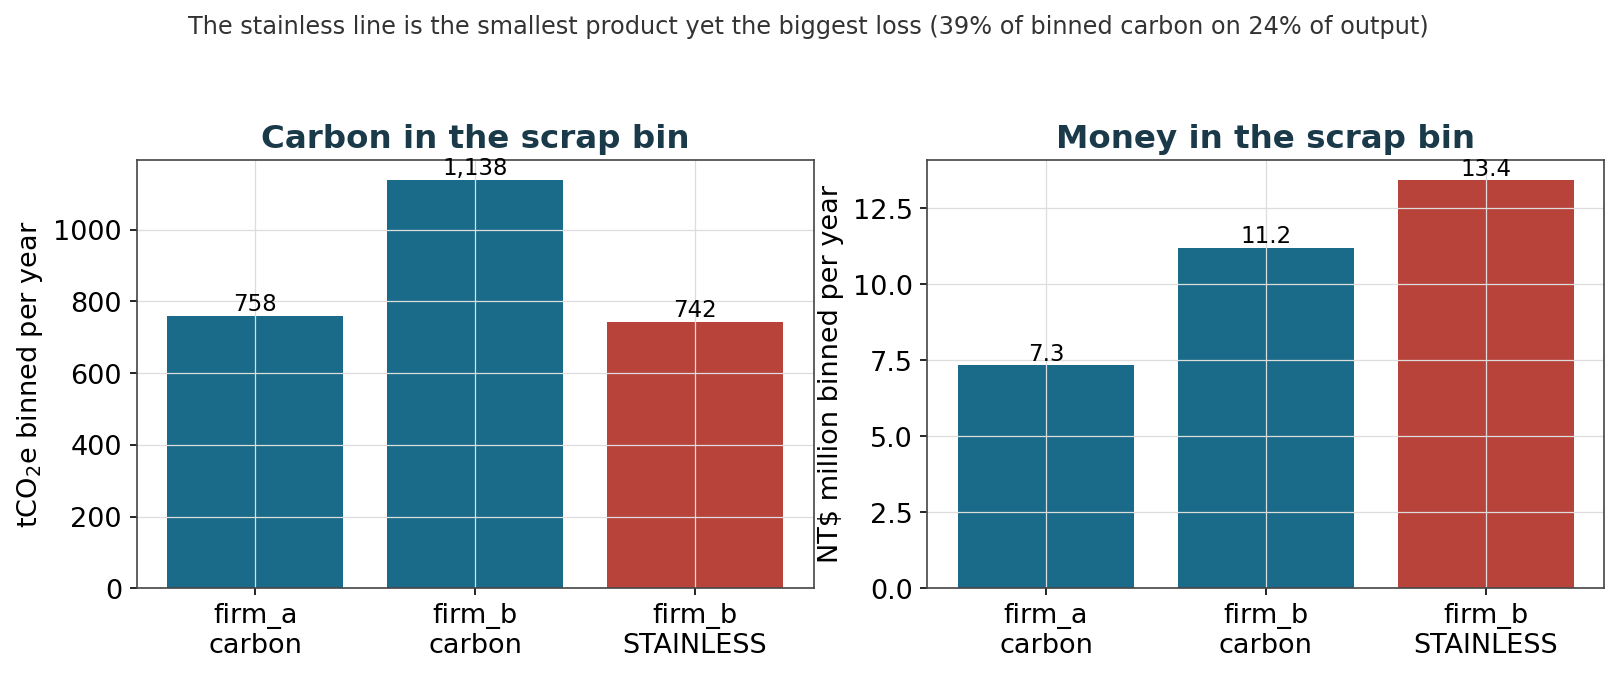
\includegraphics[width=0.96\textwidth]{charts/chartA_waste.png}
\caption{The stainless line is the \emph{smallest} product yet the largest single loss --- 39\% of the firm's binned carbon on 24\% of its output --- because a tonne of scrapped stainless carries $\sim$2.1$\times$ the carbon and $\sim$3.9$\times$ the money of carbon steel (from the invoices)\cite{repo}.}
\label{fig:waste}
\end{figure}

\subsubsection*{Why this is the right lever, not the grid}
Because the scrap sits inside the declared number, cutting it is the only reduction we built that \emph{also} lowers the CBAM figure. Table~\ref{tab:levers} and Figure~\ref{fig:levers} put it beside the grid-aware scheduler we also implemented and measured.

\begin{table}[htbp]
\caption{Two reduction levers for Firm A, engine-measured}
\label{tab:levers}
\small
\begin{tabularx}{\textwidth}{@{}Xrrl@{}}
\toprule
\textbf{Lever} & \textbf{tCO$_2$e/yr} & \textbf{\NT/yr} & \textbf{Moves the CBAM number?} \\
\midrule
Yield: 9.1\%\,$\to$\,5\% loss & \textbf{359} & 3.48\,M & \textbf{Yes} --- SEE 2.924\,$\to$\,2.805 ($-$€9.01/t, $-$€27{,}040/yr) \\
Grid-aware load shifting (Module 2) & 4.49 & 0.40\,M & No --- indirect emissions are out of scope for CN 7318\cite{qa} \\
\bottomrule
\end{tabularx}
\end{table}

\begin{figure}[htbp]\centering
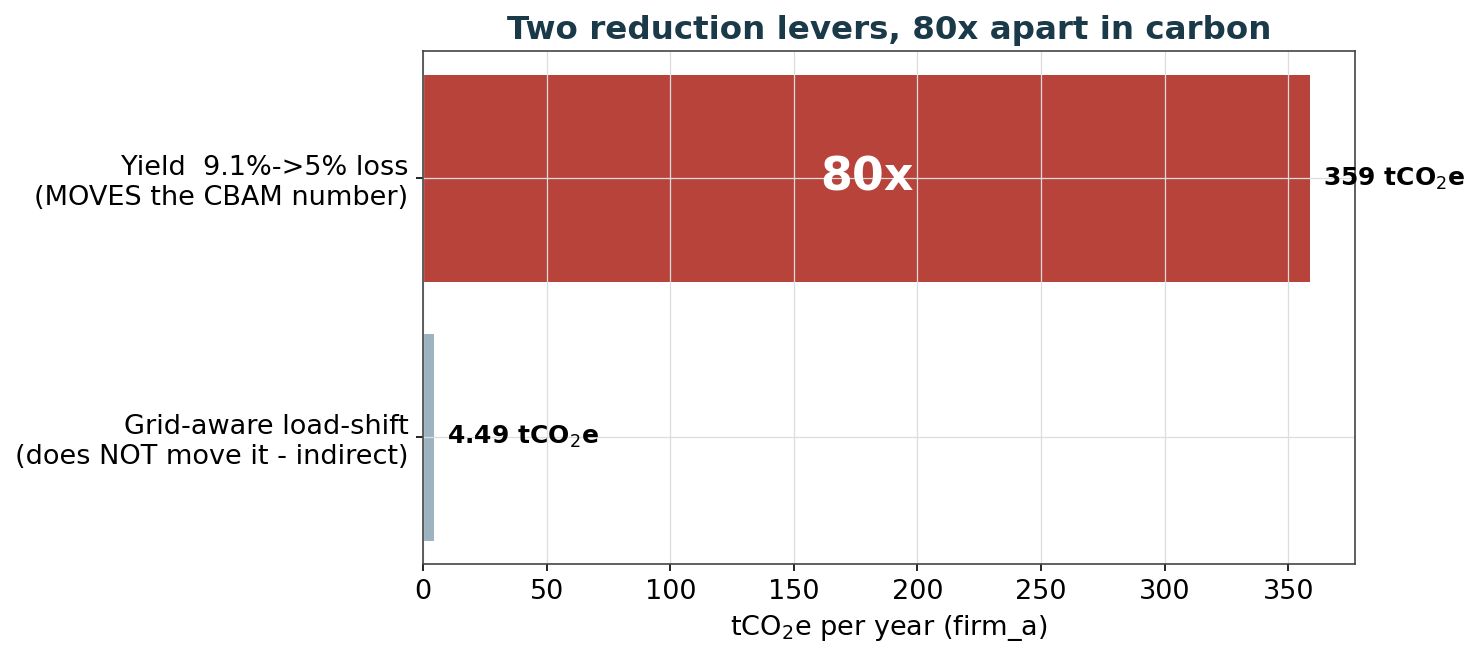
\includegraphics[width=0.82\textwidth]{charts/chartB_levers.png}
\caption{The yield lever carries roughly eighty times the carbon of the scheduling module --- and it is the one that moves the compliance number. We built a scheduler that saves 4.49 tonnes a year while the same factory put 758 in a skip, and never looked.}
\label{fig:levers}
\end{figure}

\subsubsection*{A person, and the divide}
Mr.~Lin, 61, Gangshan: thirty employees, a back office that is his daughter-in-law and a spreadsheet. To see Table~\ref{tab:waste} he would have to reconcile twenty-two steel e-invoices across twelve months against a production log, per customs code, knowing that carbon wire rod carries 2.53 tCO$_2$e per tonne. His 3,000-employee competitor in the same district sees this on a dashboard, weekly. Mr.~Lin has never seen it once. That is the divide, in the Handbook's own three axes: \textbf{ages} (an analog-native owner, no data professional in the building), \textbf{regions} (Gangshan--Luzhu, $\sim$1,800 firms of this shape), \textbf{needs} (not ``market access'' in the abstract but \textbf{\NT3.5\,million and 359 tonnes of CO$_2$ a year he cannot see}). The AI is why the gap closes rather than being merely described: the capability that costs a corporation an ERP licence costs Mr.~Lin a photograph.

\subsubsection*{The context that keeps us honest: Taiwan's default is mild}
We say this before a judge can. Running our engine over the EU's adopted per-country tables\cite{ir2621}, Taiwan's carbon-steel fastener default ($\approx$€224/t in 2026) is unremarkable --- far below China, India, T\"urkiye or Indonesia (Figure~\ref{fig:comp}); independent trade press prices it the same way (Taiwan €150/t vs T\"urkiye €400, China €500)\cite{crowe}. CBAM is, for carbon steel, a tariff on Taiwan's \emph{competitors}' inability to prove their numbers. That is precisely why Taiwan is the lab and not the victim --- and why a project that merely optimised a Gangshan exporter's margin would not matter. The waste finding is what makes it matter.

\begin{figure}[htbp]\centering
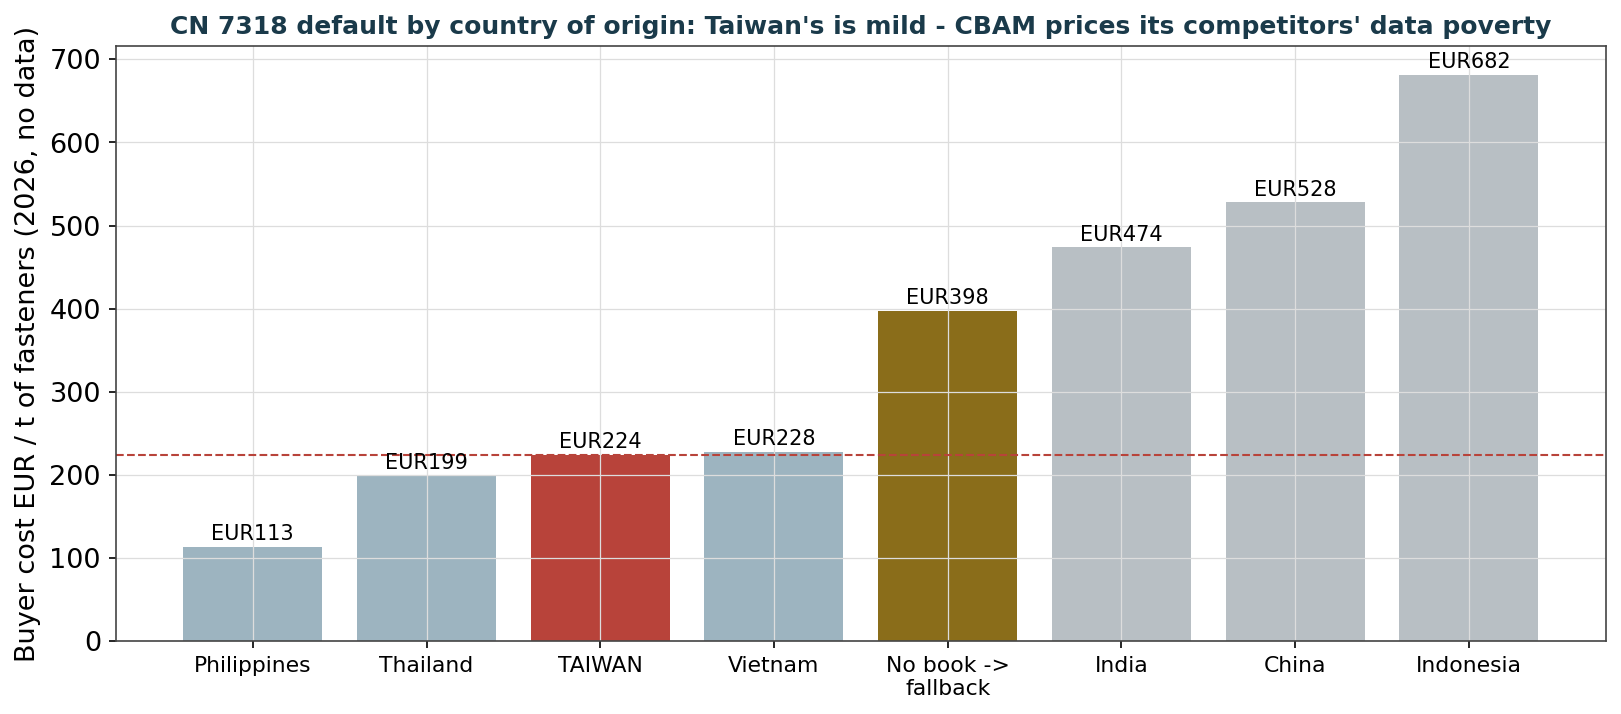
\includegraphics[width=0.95\textwidth]{charts/chartC_competitors.png}
\caption{CN 7318 marked-up default by country of origin, 2026, at the €75.28 certificate price. Countries with no entry in the EU's book at all are priced at the ``average of the ten dirtiest exporters'' fallback\cite{qa}. Taiwan sits low; the harm is heaviest where the capacity to prove is lowest.}
\label{fig:comp}
\end{figure}

\subsubsection*{The problem Taiwan cannot see: stainless}
The same scan surfaced something sharper. Taiwan's stainless steel is among the most carbon-intensive on earth ($\sim$2.6$\times$ the world median), yet the EU gives a stainless fastener the \emph{same} carbon-steel default (2.707 tCO$_2$e/t) --- and the stainless rod a fastener plant actually buys (CN 7221) has \emph{no Taiwanese value in the EU's table at all}, sending it to the punitive fallback. For Firm B's stainless line, honest reporting would raise the buyer's cost by \textbf{€228/t --- €296,006 a year} (Figure~\ref{fig:ss}, Table~\ref{tab:ss}). So nobody reports it, and Taiwan's worst carbon problem stays legally invisible. A filing tool tells the stainless maker to stay quiet. A \emph{waste} tool tells him the stainless in his scrap bin is the most expensive thing he throws away --- true, actionable, and worth it to him whatever he files.

\begin{table}[htbp]
\caption{Stainless fastener, Firm B: the default hides the emissions}
\label{tab:ss}
\small
\begin{tabularx}{\textwidth}{@{}Xrrl@{}}
\toprule
\textbf{Basis} & \textbf{tCO$_2$e/t} & \textbf{Buyer pays} & \textbf{Note} \\
\midrule
EU default used today (a carbon-steel number) & 2.978 & €224/t & a $\sim$2.0$\times$ under-count \\
Honest actual (correct CN 7221 precursor + fallback) & 6.003 & €452/t & $+$€228/t $=$ €296,006/yr \\
\bottomrule
\end{tabularx}
\end{table}

\begin{figure}[htbp]\centering
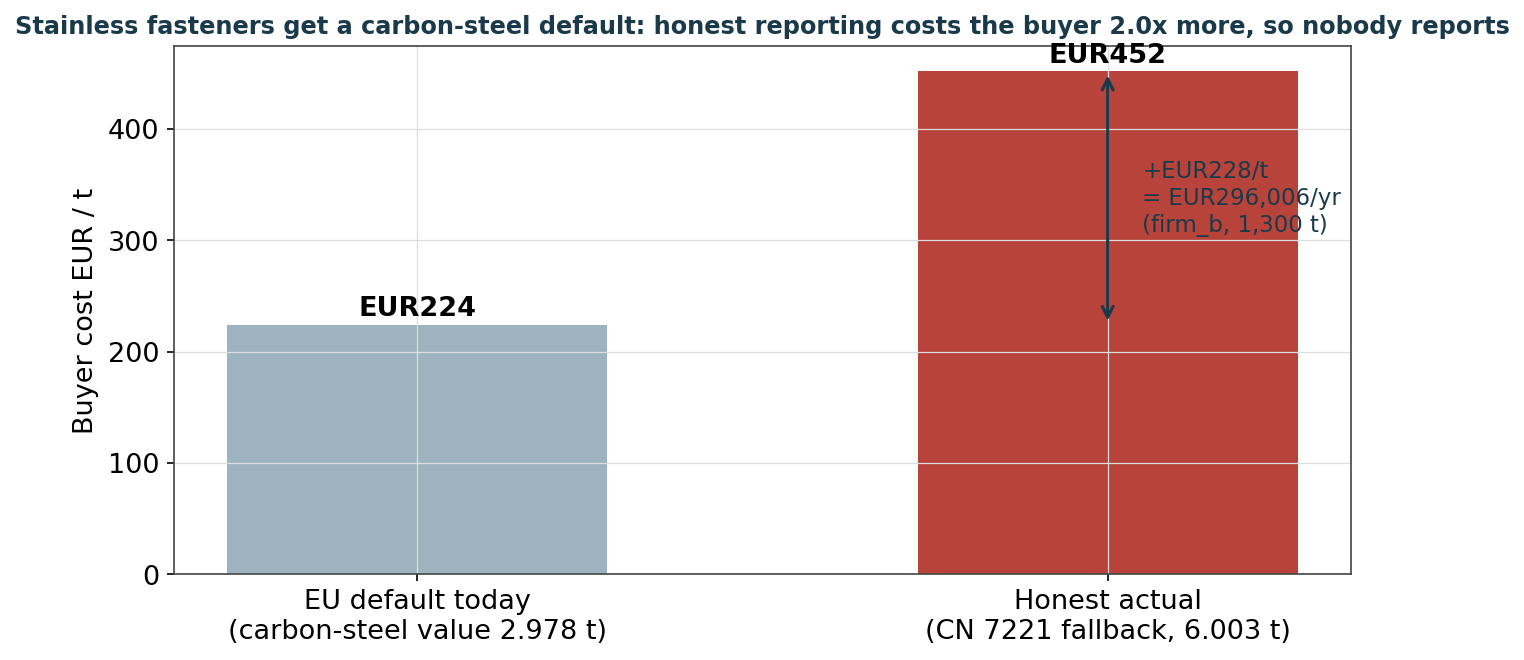
\includegraphics[width=0.72\textwidth]{charts/chartD_stainless.png}
\caption{Honest reporting of a Taiwanese stainless fastener costs the buyer twice as much as the default --- the incentive is to stay silent, which is exactly why the emission stays invisible and unfixed.}
\label{fig:ss}
\end{figure}

\subsection{Related stakeholders and their roles}
The \textbf{target audience is the fastener SME owner} --- lowest digital readiness, highest concentration, and the person the waste map actually pays. Table~\ref{tab:stake} lists the chain.
\begin{table}[htbp]
\caption{Stakeholders and roles (target audience in bold)}
\label{tab:stake}
\small
\begin{tabularx}{\textwidth}{@{}lX@{}}
\toprule
\textbf{Stakeholder} & \textbf{Role and benefit} \\
\midrule
\textbf{Fastener SME owners (target)} & Primary users: recover money and carbon from scrap; obtain the buyer's data pack in their own language \\
EU importers / declarants & Receive template-ready supplier data; avoid punitive fallback defaults\cite{qa} \\
TIFI ($\sim$700 members) \& MIRDC & Pilot recruitment, real cluster yield data, rollout channel \\
MOENV / Climate Change Admin & Their CBAM platform gains the computation and waste layer it lacks; 20 idle verification bodies\cite{moenv} \\
MOEA / SMESA & Execution tool for SME competitiveness programmes \\
Taiwan Power Company & Open data (10-min feed, TOU) becomes value-generating for small industry \\
Accredited verifiers & Structured, uncertainty-annotated input instead of raw paper \\
\bottomrule
\end{tabularx}
\end{table}

\subsection{Description of the solution's functions}
\textbf{One photograph, two outputs.} Mr.~Lin sends a photo of his Taipower bill and his steel e-invoices to a LINE chat in Taiwanese. Within about ninety seconds he receives: the \textbf{CBAM data pack} for his screws, per customs code, in the European Commission's own template, flagged actual/default with per-line uncertainty (the artifact the buyer asks for); and the \textbf{waste map} --- \emph{``this year you binned 758 tonnes of CO$_2$ and \NT7.35\,million of steel; here is which line, and here is what 5\% loss would return.''} No portal, no consultant, no data leaving his building.

\begin{table}[htbp]
\caption{Pipeline: the door-opener and the product from one ingestion}
\label{tab:pipe}
\small
\begin{tabularx}{\textwidth}{@{}lX@{}}
\toprule
\textbf{Stage} & \textbf{What happens} \\
\midrule
Inputs he already has & Taipower bill (photo) $+$ steel e-invoices (e-GUI XML) $+$ production log \\
Ingestion (offline) & \texttt{qwen3-vl} 4B parses to validated activity data; a second OCR pass cross-checks every number \\
Compliance branch & allocation $\to$ SEE engine $\to$ filled EU template $+$ default-vs-actual buyer screen \\
\textbf{Waste branch} & yield per line per CN code $\to$ carbon and \NT{} in the scrap $\to$ reduction ranking \\
\bottomrule
\end{tabularx}
\end{table}

\subsection{Differences from existing solutions}
Every existing instrument --- the government CAAS portal, the MOEA calculator, the MOENV CBAM platform, private ESG SaaS, consultants --- computes a carbon number in order to \emph{file} it. \textbf{CarbonPass computes it in order to \emph{cut} it.} The yield lever falls straight out of the Commission's own SEE formula, where nobody looked because they read it as an accounting rule rather than an optimisation target. No existing tool converts SME-native documents into a per-line waste map at near-zero marginal cost, in the owner's language, offline. And nothing else runs the whole ingestion on a \textbf{4B model on a laptop with no GPU} --- which is not an efficiency footnote but the entire inclusion claim: AI on the excluded side of the wall.

\subsection{Expected benefits (quantified)}
\begin{table}[htbp]
\caption{Expected benefits, with basis}
\label{tab:benefits}
\small
\begin{tabularx}{\textwidth}{@{}Xl@{}}
\toprule
\textbf{Benefit} & \textbf{Quantification (basis)} \\
\midrule
Waste made visible (Firm A) & 758 tCO$_2$e $+$ \NT7.35\,M/yr in scrap; Firm B: 1,879 tCO$_2$e $+$ \NT24.6\,M/yr (engine)\cite{repo} \\
Yield improvement (Firm A, 9.1\%$\to$5\%) & 359 tCO$_2$e/yr; lowers SEE 2.924$\to$2.805; \NT3.48\,M/yr (engine)\cite{repo} \\
Stainless emission surfaced (Firm B) & 742 tCO$_2$e/yr on the smallest line; €296,006/yr honesty gap the default hides\cite{repo} \\
Energy cost (secondary, Module 2) & \NT399,800/yr on shiftable loads --- the ``bill module'', not the carbon module\cite{repo} \\
Compliance labour & a photograph and $\sim$90\,s vs consultant-weeks; recurring at near-zero marginal cost \\
Population at beachhead & $\sim$1,800 cluster firms, each binning $\sim$10\% of its steel; 2,600 CBAM-exposed SMEs\cite{moenv} \\
\bottomrule
\end{tabularx}
\end{table}

% ===== 3 MATURITY =====
\section{Maturity, Implementation and Verification}\label{sec:maturity}

\subsection{Development stage --- what already runs}
An early prototype built for this competition, not commercialised. Working today, reproducible from the repository: the ingestion pipeline; the allocation engine (uncertainty $\pm$1.06\% 1$\sigma$); the SEE rules engine (Commission worked example reproduced at rel $10^{-9}$); the template writer (a real 19-sheet Commission workbook filled, its SEE cells independently recomputing in LibreOffice to the engine's sidecar at $\sim$$10^{-11}$); the waste analyser (run on two firms); the grid-aware scheduler on Taipower's live 10-minute feed; and a LINE interface with a credential-free simulator. \textbf{The full test suite is green (25/25).}\cite{repo} The compliance core is already general: the engine parsed 120 country sheets and 12{,}532 default rows with zero failures\cite{repo}.

\begin{figure}[htbp]\centering
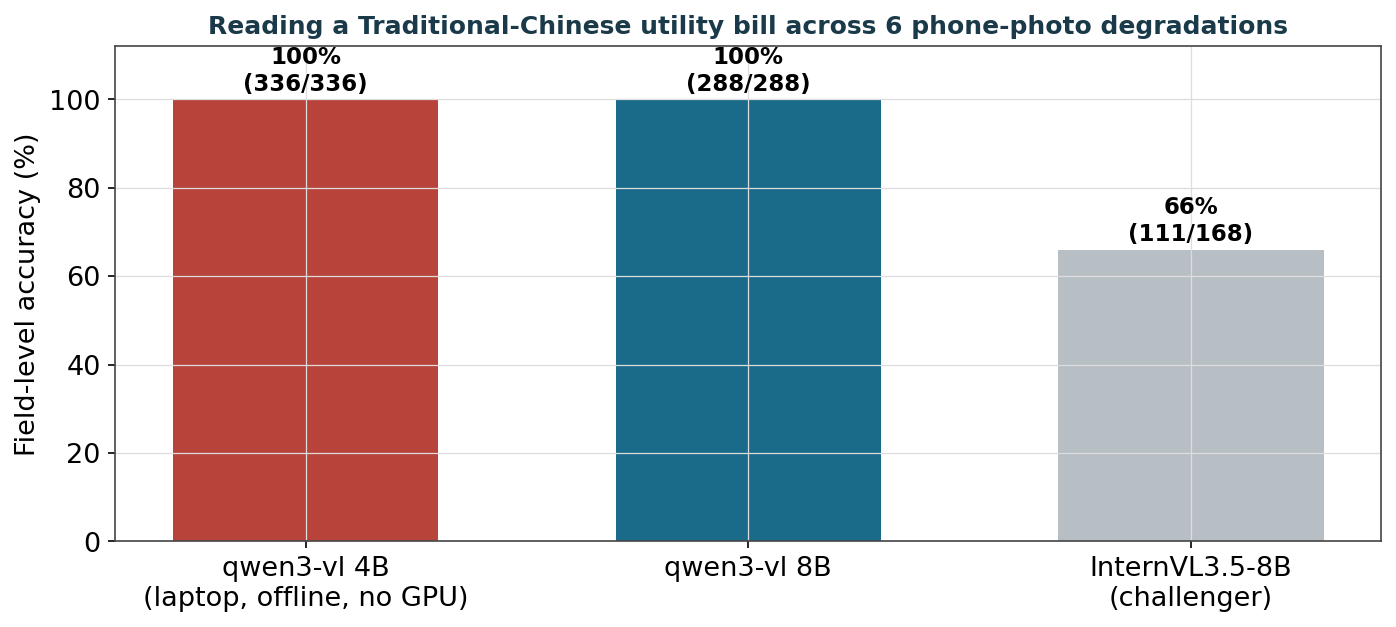
\includegraphics[width=0.80\textwidth]{charts/chartE_vlm.png}
\caption{Sprint-1 model bake-off on degraded phone photos. The 4B tier matches the 8B and beats the approved challenger, at lower latency --- validating the offline, no-GPU inclusion tier\cite{repo}.}
\label{fig:vlm}
\end{figure}

\subsection{Validation plan, on the campaign's own calendar}
\begin{table}[htbp]
\caption{Implementation \& verification milestones}
\label{tab:plan}
\small
\begin{tabularx}{\textwidth}{@{}lX@{}}
\toprule
\textbf{Window (Handbook)} & \textbf{Milestone} \\
\midrule
By 31 Jul 2026 (submission) & Working PoC + demonstration video (the LINE simulator makes it recordable today); outreach to TIFI, MIRDC, Kaohsiung EPB \\
Mid-Sep -- mid-Oct (mentorship) & One pilot factory in Gangshan: real bills in, real pack and \textbf{real yield curve} out; MIRDC/verifier review; first \emph{observed} cluster loss figures \\
Late Oct (final review) & Live demo: pack, waste map, and a measured before/after yield on one line; market outlook updated with the Sept verifier-accreditation and EP downstream-scope developments \\
\bottomrule
\end{tabularx}
\end{table}
Two natural experiments fall inside the window: the first CBAM verifier accreditations are expected $\sim$September 2026, and the European Parliament vote on the $\sim$180-category downstream extension is expected the same month\cite{moenv,qa}.

\begin{formfield}{Boundaries stated up front (see also \S7)}
Scrap is recycled and remelted, so the \emph{compliance} (SEE) effect is exact and 1:1, but the \emph{atmospheric} effect is smaller than the gross tonnage --- remelting recovers the iron, not the energy already spent making the rod. We always state the gross figure with this caveat and never claim tonnes ``avoided''. Yield magnitudes (9.1\%) are from a synthetic corpus: the mechanism is certain, the magnitude needs the pilot. The tool tells the owner \emph{that}, \emph{where}, and \emph{what it is worth}; it does not yet claim to tell him \emph{how} to cut it. Filing alone is worth $\approx$€4/t to a Taiwanese carbon-steel maker --- which is why the pack is the door-opener and the waste is the value.
\end{formfield}

% ===== 4 FUTURE =====
\section{Future Plans}\label{sec:future}
\textbf{2026--2027 (Taiwan).} Harden the pilot into a cluster rollout via TIFI/MIRDC; publish the give-back datasets (\S5); propose integration of the waste-and-computation layer into MOENV's CBAM platform and SMESA's service network. \textbf{2027--2028 (surface the invisible).} Take the stainless finding to MOENV and the Commission (a missing CN 7221 value is worth more to Taiwan than to us); extend the same engine to the downstream categories if the EP confirms the extension. \textbf{2028+ (Taiwan can help).} The instrument is built to travel: ASEAN and South Asia foreground, where exporters face the punitive fallback with far thinner tooling than Taiwan's, aligned with the New Southbound policy. Everything already built --- ingestion, allocation, SEE engine, writer, scheduler, LINE, the 4B edge tier --- is re-aimed, not rebuilt.

% ===== 5 OPEN DATA =====
\section{Open Data}\label{sec:opendata}
\textbf{Used:} MOENV carbon-footprint coefficients (data.gov.tw \#28176; 1{,}164 rows in repo); the EU's adopted default-value\cite{ir2621}, methodology\cite{ir2547} and benchmark tables; Taipower's 10-minute generation feed (\#8931) and TOU schedules; MOF e-invoice (電子發票 / MIG 4.0). \textbf{Suggested improvements (form field):} our engine found real defects in the EU's own published tables --- 87 of 120 country sheets carry no fastener row and reach the punitive fallback by omission; three different dash characters and inconsistent CN formatting silently break joins; and CN 7221 (stainless rod) is missing for exactly the three fastener exporters (Taiwan, Thailand, Vietnam). \textbf{Given back:} (1) a \textbf{fastener-sector yield benchmark} --- the first of its kind, worth more to the cluster than any grid dataset because it tells each firm whether its 9.1\% is good; and (2) a cleaned, defect-annotated \textbf{machine-readable edition of the CBAM default and benchmark tables} with the coverage map, published open.

% ===== 6 OPEN SOURCE =====
\section{Open-Source Software Design}\label{sec:oss}
Built on open components (an Apache-2.0 vision-language model, open optimisation and spreadsheet libraries). The team intends to release the compliance rules engine, the waste analyser and the cleaned atlas under an open licence, and is willing to allow future open-source use --- consistent with the competition's encouragement\cite{handbook}. \emph{(Per the Handbook, this section does not affect the score.)}

% ===== 7 HONEST LIMITS =====
\section{Honest Limits and Scope Discipline}\label{sec:limits}
These are carried into every artifact, not buried.
\begin{enumerate}[leftmargin=1.3em,itemsep=1.5pt]
\item \textbf{Recycling caveat.} Scrap is remelted: SEE effect exact 1:1 (CBAM counts mass before cutting\cite{qa}); atmospheric effect smaller than gross. State both; never claim tonnes ``avoided''.
\item \textbf{Synthetic magnitude.} 9.1\% is from a generated corpus; real cluster yields are the first thing to ask MIRDC/TIFI for. 5\% is a scenario, not a promise.
\item \textbf{No process claims.} We show that/where/what-worth, not yet how; die life, setup scrap and coil-end optimisation are pilot domain problems.
\item \textbf{Stainless, verified once.} Figures are the corrected CN 7221 basis ($\sim$2.16$\times$, $+$€228/t, 742 tCO$_2$e); a ``see below'' with nothing below it may be a publishing defect --- to be confirmed against the legal text\cite{ir2621} before the ``hole in the book'' is asserted as intent.
\item \textbf{Taiwan's mildness is a feature.} Its default is low; that is the reason for a global architecture, not an embarrassment.
\item \textbf{The verification market is opaque.} No CBAM verification price is published anywhere; we do not invent one. Only four of twenty-four EU accreditation bodies accept third-country applications and \emph{zero} CBAM verifiers are accredited as of July 2026\cite{ecacc} --- the absence is the argument, and the claim is scoped to the year-one cold start.
\item \textbf{Engine scope.} Every figure here is steel; cement and fertiliser await two documented fixes before publication.
\end{enumerate}
\textbf{Retired claims (never reused):} the ``€450--750/t default'' and ``30--50\% of product value'' folklore (false for Taiwan --- it described the fallback and the dirtiest origins); an ``80\%-actual / 20\%-default'' rule and a ``5\% variance threshold'' (in no adopted text); ``developing countries get worse defaults'' (false by our own measurement --- both tails are developing economies); and ISO~14067 as a CBAM by-product (LCA factors are not accepted for CBAM\cite{qa}).

\begin{spotlight}{The claim, in one line.}
The EU did not build a machine that taxes carbon; it built one that taxes \emph{proof} --- and the same photograph that produces the proof reveals the tenth of the steel a small factory throws away, which it has never once been able to see. Taiwan does not have the injury. Taiwan has the answer.
\end{spotlight}

% ===== REFERENCES =====
\clearpage
\phantomsection\addcontentsline{toc}{section}{References}
\footnotesize
\begin{thebibliography}{99}\setlength{\itemsep}{2.2pt}
\bibitem{qa} European Commission, DG TAXUD. \emph{CBAM Questions and Answers} (definitive period), 27--28 May 2026 --- default values usable for all non-electricity goods (p.36 \S4.25), mass before cutting (p.32 \S4.11), iron/steel scope is direct-only (p.34 \S4.16), fallback = ten highest-intensity exporters (p.37 \S4.26), LCA factors not accepted (p.36 \S4.24). \href{https://taxation-customs.ec.europa.eu/carbon-border-adjustment-mechanism/cbam-communication-and-faqs_en}{taxation-customs.ec.europa.eu}
\bibitem{ir2621} Commission Implementing Regulation (EU) 2025/2621 (default values), 16 Dec 2025, and the adopted machine-readable table ``DVs as adopted v20260204''. Taiwan CN 7318 direct default = 2.70719 tCO$_2$e/t. \href{https://eur-lex.europa.eu/legal-content/EN/TXT/?uri=OJ:L_202502621}{eur-lex.europa.eu}
\bibitem{ir2547} Commission Implementing Regulation (EU) 2025/2547 (methods for calculating embedded emissions), 10 Dec 2025. \href{https://eur-lex.europa.eu/legal-content/EN/TXT/?uri=OJ:L_202502547}{eur-lex.europa.eu}
\bibitem{repo} CarbonPass engine and analysis (this project), 17 Jul 2026 --- all figures reproducible: \texttt{atlas\_scan.py}, \texttt{waste\_scan.py}, \texttt{vlm\_bakeoff.py}, golden tests (rel $10^{-9}$), LibreOffice recompute check, 25/25 tests green.
\bibitem{crowe} McLeod, J. (Crowe UK). ``The new reality of CBAM.'' \emph{Fastener + Fixing Magazine}, 9 Feb 2026 --- heading 7318 defaults: Taiwan €150/t, T\"urkiye €400/t, China €500/t; actual data €50--100/t.
\bibitem{moenv} Ministry of Environment (Taiwan), \emph{Major Environmental Policies}, March 2026 --- 20 domestic GHG verification bodies, 200+ specialists, zero EU applications, EU-side blockers; $\sim$2,600 exposed steel-product SMEs, 3.74\,Mt, 13th-largest CBAM exporter. \href{https://www.moenv.gov.tw/en/}{moenv.gov.tw}
\bibitem{ecacc} European Commission, DG TAXUD, ``State-of-play CBAM accreditation'' (retrieved 17 Jul 2026) --- of 24 national accreditation bodies, 11 ready and 4 accepting third-country applications (Italy, Netherlands, Poland, Sweden); zero CBAM verifiers accredited worldwide as of July 2026. \href{https://taxation-customs.ec.europa.eu/carbon-border-adjustment-mechanism/cbam-verification_en}{taxation-customs.ec.europa.eu}
\bibitem{handbook} Ministry of Digital Affairs / Taipei Computer Association. \emph{2026 Presidential Hackathon International Track Handbook}, May 2026. \href{https://presidential-hackathon.taiwan.gov.tw/en/international-track/}{presidential-hackathon.taiwan.gov.tw}
\end{thebibliography}
\end{document}
